\ifx\headerIncludedJR\undefined
  \documentclass[11pt,a4paper]{article}
  \setlength{\textwidth}{5.50in}
  \usepackage[utf8]{inputenc}
\usepackage[T1]{fontenc}
\usepackage{amsmath}
\usepackage{amsthm}
\usepackage{amssymb}
%\usepackage{rotating}
%\usepackage{amslatex}
\usepackage{siunitx}
\usepackage{multicol}%for multicol
\usepackage{blkarray}%blockarray and block
\usepackage{comment}
\usepackage{fnbreak}%get a warning if a footnote is split
\usepackage[section]{placeins}
\usepackage{listings}
\lstset{breaklines=true,basicstyle=\ttfamily,language=Python}
\usepackage{arrayjobx}
\usepackage{array}%for \newcolumntype
%\usepackage[shortlabels]{enumitem}
\usepackage{mathtools}
\usepackage{afterpage}
\usepackage{setspace}% for \setstretch
\usepackage{algorithm}
\usepackage{algpseudocode}%for algorithmic
\usepackage{thmtools}%so that autoref works with Lemmas
\usepackage{tikz}
\usepackage{pgfplots}
\pgfplotsset{compat=1.15}
\usepackage{shuffle}
\usepackage{textcomp}%for \textrecipe
\usepackage{fontawesome}%for \faTable
\usetikzlibrary{calc,shapes,arrows.meta,decorations.markings,arrows}
\usetikzlibrary{graphs,positioning,svg.path,backgrounds}
\newcommand{\tikzmark}[1]{\tikz[overlay,remember picture] \node (#1) {};}
%\usepackage{CJKutf8}%for CJKChar

%\usepackage[backend=biber,backref=true]{biblatex}
\usepackage[backend=biber,style=alphabetic,backref=true,maxbibnames=10]{biblatex}
\addbibresource{sigs.bib}
\usepackage{url}

\usepackage{imakeidx}
%not a list of definitions, just symbols and abbreviations
%What is an abbreviation? Is QR? 
\makeindex[intoc,title=Symbols and abbreviations index]
\def\jind#1{\index{#1}}
\def\jindmath#1#2{\index{#2@$#1$}}
\def\jindv#1{\index{#1v@\texttt{#1}}}
%Some places I've given up and used \index in the text 
\definecolor{bluee}{rgb}{0.4, 0.4, 1.0}
%https://tex.stackexchange.com/questions/134191/line-breaks-of-long-urls-in-biblatex-bibliography
\setcounter{biburlucpenalty}{8000}
\setcounter{biburllcpenalty}{8000}

\usepackage{hyperref}

%so that autoref works with algorithms
\newcommand{\algorithmautorefname}{Algorithm}

%might help url breaking in bibliography
%\Urlmuskip=0mu plus 1mu minus 1mu
%also all the emergencystretch/looseness/fussy/sloppy
%to play with
%https://tex.stackexchange.com/questions/18505/how-to-use-sloppy-for-just-some-references

\def\ii{{\texttt{iisignature}}}
\def\pypi{{\texttt{PyPI}}}
\def\numpy{{\texttt{numpy}}}
\def\scipy{{\texttt{scipy}}}
\def\i#1{\index{#1@\texttt{#1}}}
\def \hilite#1{\underline{\color{blue}\textbf{#1}}}
%\def \alph#1{{\color{blue}\mathbf{#1}}}
\def \lex{<_L}
\def\kron{\underline{\otimes}}

\graphicspath{{C:/Users/Jeremy/Dropbox/phd/graphs/}{/home/jeremyr/Dropbox/phd/graphs/}{/Users/reizenstein/DropboxPersonalSymlink/phd/graphs/}}

%\RequirePackage{relsize}
%\DeclareRobustCommand\CXX{C\kern-.05em \raisebox{.3ex}{\scalebox{0.9}{\textbf{+\kern-.10em+}}}}
\DeclareRobustCommand\CXX{C\kern-.05em {\scalebox{0.9}{\textbf{+\kern-.10em+}}}}
%\DeclareRobustCommand\{\texorpdfstring{\CXX}{C++}}
\DeclareRobustCommand\CC{C\texttt{++}}
\def\bftab{\fontseries{b}\selectfont}
\newtheorem{theorem}{Theorem}
%\newtheorem*{theorem*}{Theorem}%bad idea, because you can't refer to it.
\newtheorem{definition}[theorem]{Definition}
%\newtheorem{outsideTheorem}[theorem]{Theorem}
\newtheorem{example}[theorem]{Example}
\newtheorem{conjecture}[theorem]{Conjecture}
\newtheorem{lemma}[theorem]{Lemma}
\newtheorem{proposition}[theorem]{Proposition}
\newtheorem{remark}[theorem]{Remark}

\newcommand{\area}{\mathsf{area}}
\newcommand{\Area}{\mathsf{Area}}
\newcommand{\emptyword}{\epsilon}
\newcommand{\ds}{d} % dimension of the signal
\newcommand{\TC}{T((\R^\ds))} % concat
\newcommand{\TS}{T(\R^\ds)} % shuffle
\newcommand{\GL}{\operatorname{GL}}
\newcommand{\SO}{\operatorname{SO}}
%\newcommand{\id}{\operatorname{id}}
\newcommand{\id}{\mathsf{id}}

\newcommand{\evaluatedAt}[1]{\,\raisebox{-.5em}{$\vert_{#1}$}}

\def\hssymbol{\mathbin{\succ}}
\def\hs#1#2{#1\hssymbol#2} %half shuffle
%\def\hs#1#2{z(#1,#2)} %half shuffle
\def\areab#1{\underline{\area}(#1)}
\def\areabb{\underline{\area}}
\newcommand{\R}{\mathbb{R}}
\newcommand{\Q}{\mathbb{Q}}
\newcommand{\C}{\mathbb{C}}
\newcommand{\N}{\mathbb{N}}
\newcommand{\spann}{\operatorname{span}}
\newcommand{\sign}{\operatorname{sign}}

\DeclareMathOperator*{\argmax}{arg\,max}
\DeclareMathOperator*{\argmin}{arg\,min}
\DeclareMathOperator{\softmax}{softmax}

%indicate that this file has been had
\def\headerIncludedJR{}
\def\endDocumentJR{}

%general hints
%https://homepages.inf.ed.ac.uk/imurray2/compnotes/latex.html

  %this cannot be in header.tex as it messes up
  %the thesis copyright page
  \def \alph#1{{\color{bluee}\mathbf{#1}}}
  \begin{document}
  \tableofcontents
  \def\endDocumentJR{\printindex \printbibliography[heading=bibintoc]\end{document}}
\fi

%\section{Introduction}
The signature is an object which is crucial in the mathematical theory of rough paths\cite{Lyons98}, and the calculations have proved to be useful in machine-learning applications, particularly classification problems where the data itself is a stream or a path in space, ranging from an application to online Chinese handwriting recognition in 2013 \cite{BEN} to skeleton-based human action recognition in 2017 \cite{action}. Other domains where the data has this form include signals from EEG and other medical monitors, sound and financial time series, where some set of numbers is varying in time. Often the samples can be noisy, can have varying length and both local and global structure can be important. A survey of such applications is given in \cite{OxSigIntro}. 
\section{Plan}
\newcommand{\jrmath}{$\square$}
\newcommand{\jralgo}{\faListOl}%needs font awesome
%\textrecipe %needs textcomp, BG says too Roman-looking, it's slightly amusing
\newcommand{\jrresults}{\faTable}%faTable needs font awesome
%\viewdata ?Checkedbox, some sort of pencil?
%?\StopWatchStart for timings?
%https://tex.stackexchange.com/questions/121865 
%https://tex.stackexchange.com/questions/400557/how-to-add-connected-graphs-to-a-table
%https://tex.stackexchange.com/questions/33787/how-do-i-create-separate-columns-in-latex-without-text-flow
%\newcommand*{\fullref}[1]{\hyperref[{#1}]{\autoref*{#1} \nameref*{#1}}}
\newcommand*{\fullref}[1]{\hyperref[{#1}]{\ref*{#1} \nameref*{#1}}}
%autoref, autopageref seem useful
%There are independent streams of progress made in this document in the use of signatures in machine learning.  
\autoref{fig:plan} indicates contributions in subsequent chapters: sections which contain mathematical results with \jrmath,
those which describe algorithms with \jralgo{}
and those containing the results of computer experiments with \jrresults. The remainder of this introductory chapter introduces the signature in more detail.

\newcommand{\tablenode}[2]{\tikz[baseline=(#1.base),remember picture]\node[inner sep=0pt,name=#1]{#2};}
\newcommand{\jrsp}{\hspace{1em}}
%\enlargethispage{3\baselineskip}
\begin{figure}[h]
%\renewcommand\arraystretch{1}
%\begin{center}
\centering
 \begin{tabular}{l}
\tablenode{t1}{\fullref{chap:math}}\\
\jrsp\tablenode{tm1}{\fullref{sec:fkk}} \jrmath\\
\jrsp\tablenode{tm2}{\fullref{sec:myInvariant}} \jrmath\\
\jrsp\tablenode{tm3}{\fullref{sec:rotinv2d}} \jrmath\ \jralgo\\
\tablenode{t2}{\fullref{chap:aoa}} \\
\jrsp\tablenode{ta1}{\fullref{sec:aoaLinearU}} \jrmath\\
\jrsp\tablenode{ta2}{\fullref{sec:aoaLinear2d}} \jrmath\\
\tablenode{t3}{\fullref{chap:iisig}}\\
\jrsp\tablenode{ti1}{\fullref{sec:sigs}} \jralgo\\
\jrsp\tablenode{ti2}{\fullref{sec:c}} \jralgo\\
\jrsp\tablenode{ti3}{\fullref{sec:s}} \jralgo\\
\jrsp\tablenode{ti4}{\fullref{sec:impl} \jralgo}\\
\jrsp\tablenode{ti5}{\fullref{sec:time} \jrresults}\\
\jrsp\tablenode{ti6}{\fullref{sec:mem} \jrresults}\\
\jrsp\tablenode{ti8}{\fullref{sec:backprop}} \jralgo\\
\tablenode{t4}{\fullref{chap:deep}}\\
\jrsp\tablenode{tc2}{\fullref{sec:chinese} \jralgo\ \jrresults\ }\\
\jrsp\tablenode{tc4}{\fullref{sec:lstmsig} \jralgo\ \jrresults\ }\\
\end{tabular}
\begin{tikzpicture}[remember picture, overlay]
\def\drawadjL#1#2{\draw [->] ($(#1.west)+(-1em,0)$) to[out=180,in=180,looseness=2  ] ($(#2.west)+(-1em,0)$);}
%\def\drawadjLD#1#2{\draw [dotted,->] ($(#1.west)+(-1em,0)$) to[out=180,in=180,looseness=2  ] ($(#2.west)+(-1em,0)$);}
\def\drawadjR#1#2{\draw [->] ($(#1.east)+(1em,0)$) to[out=0,in=0,looseness=2  ] ($(#2.east)+(0.5em,0)$);}
\drawadjL{ta1}{ta2}
\drawadjL{ti1}{ti4}
\drawadjL{ti2}{ti4}
\drawadjL{ti3}{ti4}
\drawadjR{ti4}{ti5}
\drawadjR{ti4}{ti6}
%\draw [dotted,->] (ti8) to[out=180,in=180,looseness=2  ] (tc2);
\begin{scope}[dotted]
\drawadjL{ti8}{tc4}
\drawadjR{ti4}{tc2}
\drawadjR{ti4}{tc4}
\end{scope}
\end{tikzpicture}
%\end{center}
  \caption[Plan of this document]{Plan of this document. Introductory sections to each chapter are omitted. Arrows indicate significant dependencies, with the dotted arrows indicating that although there is a logical dependency, the sections can be read independently. The fact the arrows are so few should be helpful.}
  \label{fig:plan}
\end{figure}

\section{What is the signature of a path?}

The iterated-integral signature of a smooth path is an infinite sequence of numbers. It is used in the mathematical theory of differential equations driven by paths. In these problems, a path is the driving signal for a certain type of system. It turns out that the signature is exactly the information about a path which you need to know in order to predict how the output of the system will behave, using a generalisation of Taylor's theorem. %solve a certain type of differential equation which depends on the path
It is natural that the signature would also be the right information to extract from a path if we want a machine-learning algorithm to understand the shape of the path.

A $d$-dimensional path is given by a function %$\gamma$ 
from an interval $[a,b]\subset\mathbb{R}$ to $\mathbb{R}^d$. 
We call $\mathbb{R}^d$ the \emph{ambient space} of the curve.
%The signature of $\gamma$ 
Its signature depends on the appearance of the path and the direction it was created, but not the speed at which it was created. If a path is modified by adding or removing a section which is exactly backtracked over, then its signature does not change \cite{HL}. If the path has a time dimension along which it always increases (for example it is the graph of a function of time) then exact backtracking is impossible and so any two different paths will have different signatures.%
\footnote{The signatures of two paths are the same iff they are \emph{tree-equivalent} \cite{HL} which means that they only differ in terms of adding or removing pieces which consist of exact backtracking.}
%\footnote{For paths which are continuously differentiable at all but finitely many places, such as the paths which we deal with in applications which are piecewise linear between a set of specified points, the signatures of two different paths which contain no exact backtracking will differ \cite{chen}. This property has been extended to general bounded variation paths by \cite{HL}, where two paths will have different signatures unless they are \emph{tree-equivalent}.}
%If two bounded variation paths are different then their signatures will be different, unless they have so-called \emph{tree-like equivalence}, which implies that at least one contains a section where the path exactly retraces itself.\cite{HL}
%\footnote{The case for paths which are continuously differentiable at all but finitely many places, which is true of the paths which we deal with in \ii, which are piecewise linear between a set of specified points which are specified by a set of points, is proved in \cite{chen}.}% The paths which we deal with in \ii, which are piecewise linear between a set of specified points, are automatically of bounded variation. %The fact that a signature cannot distinguish between two paths where the only difference is that one path contains an extra section which is backtracked over is due. %It is difficult for a writer to backtrack precisely, and so every character should be distinguishable through its signature.
%It is possible that approximate backtracking might lead to numerically unstable signatures.
%is this true?

The signature is divided into units called levels. We cannot store the whole signature of a path on a computer, rather we calculate a certain number of levels of it. 
The more levels of a signature are known, the more precisely the shape of the path is determined.
%Similar smooth curves have similar signatures.
If a path changes very slightly, the first few levels of its signature will also only change very slightly. If a path is moved (translated) but retains its shape, its signature will not change. 

%\subsubsection*{Simple example}
The number of elements of level $m$ of the signature of a $d$-dimensional path is $d^m$. They are the values of iterated integrals which consist of $m$ nested integrals, and they are labelled with $m$ numbers each corresponding to one of the dimensions. To distinguish these numbers which label the dimensions from other numbers, we write them bold and in blue. For example, a two-dimensional path might be given in coordinates as  $(\gamma_{\alph1}(t),\gamma_{\alph2}(t))$ as $t$ varies from $a$ to $b$. Its signature is a function denoted by $X^\gamma_{a,b}$\jindmath{X^\gamma_{a,b}}{X} from words made of the bold blue alphabet to real numbers. Level three of its signature has eight elements, called $X_{a,b}^\gamma(\alph{111})$, $X_{a,b}^\gamma(\alph{112})$ and so on. The one indexed by the word $\alph{122}$ is %written as
\begin{align}
X_{a,b}^\gamma(\alph{122})=\int_{t_1=a}^b\int_{t_2=a}^{t_1}\int_{t_3=a}^{t_2}d\gamma_{\alph1}(t_3)\,d\gamma_{\alph2}(t_2)\,d\gamma_{\alph2}(t_1).
\end{align}


In general, the signature can be defined inductively on the length of the word, as an element of one level of the signature of a path is an integral involving the signature of a varying portion of the path. The signature of the empty word is the single value in level 0, and it is defined to always be 1. If $w$ is a word and $i\in\{\alph{1},\alph{2},\dots,\alph{d}\}$ then $X^\gamma_{a,b}(wi)$ is defined as the Stieltjes integral $\int_a^bX^\gamma_{a,t}(w)\,d\gamma_i(t)$. In the simple case that $\gamma_i$ is differentiable, this is equal to $\int_a^bX^\gamma_{a,t}(w)\,\gamma_i'(t)\,dt$.
We also use the symbol $S(\gamma)_{a,b}$ for $X^\gamma_{a,b}$\index{S@$S(\gamma)$ and $S(\gamma)_{a,b}$}.
When the endpoints $(a,b)$ of a path $\gamma$ are clear, the signature $X^\gamma_{a,b}$ may be denoted $S(\gamma)$.%\jindmath{S(\gamma)}{S}.%
\footnote{Sometimes in analysis, the term \emph{signature} is used in a slightly different sense: the signature of a path $\gamma$ is the whole function $(c,d)\mapsto X_{c,d}^\gamma$, or something equivalent to it, not just that function's value on the path's endpoints.
%, and it is often denoted by $\mathbb{X}$ with the path denoted by $X$. 
This document does not use that sense of the word.}

The information in the first level of the signature is the total displacement of the path, i.e.~the direction and distance from its starting point to its ending point. The information which the second level of the signature adds is the \emph{signed area} of the path projected in each plane. Higher levels of the signature provide more detailed information about the path's shape.

%\subsection{More technical remarks about the signature}
%The signature is invariant on translations of the path. It is also invariant on reparametrizing the path. It may therefore be useful in defining a good representation function.
%The beginning of every signature is its zeroth level, which is always the number 1. Because this carries no information about the path, we are only concerned with the non-constant part of the signature, i.e.~all the rest. \ii\ never outputs this constant 1.


%\subsubsection*{Parsimonious definition}

%A path in $\mathbb{R}^d$ (with coordinate axes $x_{\alph1},x_{\alph2},\ldots,x_{\alph d}$) can be described by a continuous map $\gamma:[a,b]\to \mathbb{R}^d$ with $\gamma(t)=(\gamma_{\alph1}(t),\gamma_{\alph2}(t),\ldots,\gamma_{\alph d}(t))$. Its \textbf{signature} is a function from words written in the alphabet $\{\alph{1},\alph{2},\dots,\alph{d}\}$ to $\mathbb{R}$, denoted by $X^\gamma_{a,b}$. %Some example words are `$\alph1$', `$\alph2\alph1$' and `$\alph1\alph2\alph1$'.
%The signature can be defined inductively on the length of the word. The signature of the empty word is defined as 1. If $w$ is a word and $i\in\{\alph{1},\alph{2},\dots,\alph{d}\}$ then $X^\gamma_{a,b}(wi)$ is defined as $\int_a^tX^\gamma_{a,t}\gamma_i'(t)\,dt$. The  restriction of the signature to words of length $m$ is the $m$th \textbf{level} of the signature. It contains $d^m$ values.

%The signature is made up of a series of levels, one for each nonnegative integer. 
%Level $m$ can be thought of as taking values in $(\mathbb{R}^d)^{\otimes m}$, which is a $d^m$-dimensional real vector space. %, and consists of the $d^m$ values of integrals of the form 
%\begin{equation}
%\int_a^b\int_a^{t_1}\dots\int_a^{t_{m-2}}\int_a^{t_{m-1}}\,dx_{i_1}(t_m)\,dx_{i_2}(t_{m-1})\,\dots\,dx_{i_{m-1}}(t_2)\,dx_{i_m}(t_1),
%\end{equation}
%$\int_a^b\int_a^{t_1}\dots\int_a^{t_{m-1}}\,dx_{i_m}(t_m)\,\dots\,dx_{i_2}(t_2)\,dx_{i_1}(t_1)$
%where each $i_j$ is allowed to range over values in $\{\alph{1},\alph{2},\dots,\alph{d}\}$.
%In this form, the signature is seen to be an element of the tensor algebra $T(\mathbb{R}^d)=\bigoplus_{m=0}^\infty (\mathbb{R}^d)^{\otimes m}$. %Chen's identity is a convolution and the signature of a line segment is an exponential series.

%\subsection{Some properties of signatures}
%The signature of a path takes values in a submanifold of the tensor algebra. Any polynomial function of the signature is actually


\subsection{Displacement}
As mentioned, the first level of the signature of a path is just that path's total displacement vector. 
This is not a complicated thing, but in certain simple cases it may contain enough information about a path, or about a section of a path, to be used further.
For example, it is enough information about handwritten digits to make a significant guess as to what the digit is. 
The Pendigits dataset \cite{pendigits} collected the traces of many people writing the digits 0 to 9. 
Figure~\ref{fig:displacement} shows the displacement of 18 of each digit on a scatterplot, we see that many like digits are clustered together.

\begin{figure}
\includegraphics[trim=0pt 10pt 0pt 0pt, clip,width=0.8\textwidth]{displacementScatter.pdf}
%\includegraphics[width=0.8\linewidth, height=0.56\linewidth]{placeholder.jpg}
\caption[Displacement of the first stroke of handwritten digits from Pendigits]{\label{fig:displacement}Displacement (i.e.~level 1 of the signature) of the first stroke of the first 18 of each handwritten digit 0 to 9 from the training data of \cite{pendigits}. 
The bounding box of each digit is scaled to $[-1,1]^2$ so that the displacement lies in $[-2,2]^2$.}
\end{figure}

\subsection{Signed area}
\label{sec:signedArea}
For a two-dimensional path, the information carried by the first two levels of the signature is the total displacement of the path (in the first level, which is two numbers) and the signed area between the path and the straight line from its beginning to end. %(in the second level, a single number, written as a coefficient of $[\alph1,\alph2]$). 
%The log signature contains just these three numbers.
In higher dimensions, the second level of the signature gives the signed area of the path projected into any plane.
Figure~\ref{fig:sig-comp} shows this information for two straight lines in the plane and their combination, which contains area. 
For $d=1$, the signature does not contain any information beyond the total displacement of the path, and is therefore not interesting. 
$d$ should be considered as at least 2 in the mathematical results of this thesis.\footnote{This is not to say that our methods are inapplicable to one-dimensional \emph{data}. There are canonical ways to produce higher-dimensional paths from a path, for example adding a time dimension or a lead-lag transformation (e.g.~\cite{OxSigIntro}).}
\begin{figure}%[H]
%	\begin{center}
\centering
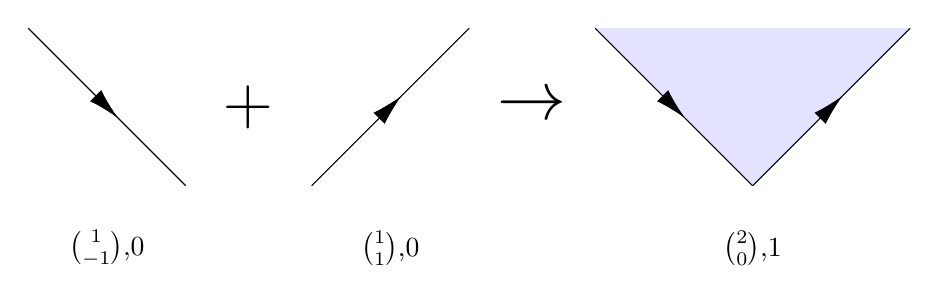
\begin{tikzpicture}

\begin{scope}[decoration={ %very thick?  thick?
	markings,
	%the xshift needs to be half the length, so that the arrow appears in the middle
	%https://tex.stackexchange.com/questions/222262/position-arrow-decoration-by-center-not-by-tip
	mark=at position 0.5 with {\arrow[xshift=2mm]{Latex[length=4mm,width=2mm]};}}
] 
\def\halfsize{1}
\def\halfskip{0.8}
\def\bottomrow{-\halfsize-\halfskip}
\def\size{\halfsize+\halfsize}
\def\startTwo{\size+\halfskip+\halfskip}
\def\startThree{\startTwo+\size+\halfskip+\halfskip}
\draw[postaction={decorate}] (0,\halfsize)--(\size,-\halfsize);
\node at (\halfsize,\bottomrow){$\binom{1}{-1}$,0};
\node at (\size+\halfskip,0) {\Huge$+$};
\draw[postaction={decorate}] (\startTwo,-\halfsize)--(\startTwo+\size,\halfsize);
\node at (\startTwo+\halfsize,\bottomrow){$\binom{1}{1}$,0};
\node at (\startTwo+\size+\halfskip,0) {\Huge$\to$};
%\fill [pattern=grid,pattern color=blue!20] %needs patterns tikzpackage
\fill [color=blue!11]
(\startThree,\halfsize)--(\startThree+\size,-\halfsize)--(\startThree+\size+\size,\halfsize)--cycle;
\draw[postaction={decorate}] (\startThree,\halfsize)--(\startThree+\size,-\halfsize);
\draw[postaction={decorate}] (\startThree+\size,-\halfsize)--(\startThree+\size+\size,\halfsize);
\node at (\startThree+\size,\bottomrow){$\binom{2}{0}$,$1$};
\end{scope}
\end{tikzpicture}
\iffalse
		\resizebox{14cm}{!}{\includegraphics{sig_from_1308_0371.pdf}}
		%\resizebox{14cm}{!}{hello I'm stuck}\resizebox{14cm}{3cm}{in a resizebox}	
%		\resizebox{14cm}{!}{
%			$1\alph1+1\alph2+0[\alph1,\alph2]$\qquad\quad $1\alph1-1\alph2+0[\alph1,\alph2]$\qquad\qquad\qquad\quad
%			$2\alph1+0\alph2-1[\alph1,\alph2]$\qquad\quad\ \ }
		\begin{minipage}{14cm}
			\hskip0pt plus0.6fil$\binom11,0$\hskip0pt plus1.2fil$\binom1{-1},0$\hfil\hfil$\binom20,-1$\hskip0pt plus0.6fil
		\end{minipage}
\fi
%		\resizebox{14cm}{!}{
%			$\qquad\binom11,0\qquad\qquad \binom1{-1},0\qquad\qquad\qquad\qquad\quad\binom20,-1\qquad\qquad\ \ $}
		%		\resizebox{14cm}{!}{
		%			$1\otimes(1,1)\otimes(\tfrac12,\tfrac12,\tfrac12,\tfrac12)$\quad\quad $1\otimes(1,-1)\otimes(\tfrac12,-\tfrac12,-\tfrac12,\tfrac12)$\qquad\qquad\quad\quad\ \
		%			$1\otimes(2,0)\otimes(2,-1,1,0)$\qquad\quad\ \ }
		%\caption{Concatenating paths and the corresponding $m=2$ log signatures, which consist of their total displacements (which are written as coefficients of $\alph1$ and $\alph2$) and the total signed area (which is written as a coefficient of $[\alph1,\alph2]$).\label{fig:sig-comp}}
		\caption[Displacement and signed areas when two lines are concatenated]{Concatenating paths and the corresponding total displacements  and total signed areas.\label{fig:sig-comp}}
%	\end{center}
\end{figure}

The following is an intuitive definition of the signed area of a path in the plane. For a smooth closed path, that is one which ends where it starts, the signed area is the sum of the signed areas of the regions bounded by the path, which is the area times the number of times the path goes round that region in an anticlockwise manner minus the number of times the path goes round it clockwise (i.e.~the winding number). For example, in the path shown in Figure~\ref{fig:winding}(a), regions whose areas count positively are labelled with a \raisebox{1mm}{\tiny\boldmath\color{red}$+$}, and negatively with a \raisebox{1mm}{\tiny\boldmath\color{red}$-$}. One region's area counts twice negatively; it is labelled with \raisebox{1mm}{\tiny\boldmath\color{red}$--$}. One enclosed region's area does not count at all, it is unlabelled. For a more general path, its signed area is the signed area of the closed path you get by joining it with a straight line from its end to its start.
\def\windingpoints{(0,0) (1,1) (3,1) (1.5,-1) (1,-1) (0.8,0.7) (1.3,1.6)(1.1,1.7)(0.9,1.4)(1.8,0.5)(2.8,-1.3)(3.6,0.2)}
\begin{figure}[H]
	\begin{center}
		\begin{tikzpicture}[font=\tiny\boldmath\color{red}]
		\begin{scope}[decoration={
			markings,
			%	mark=at position 0.08 with {\arrow{Latex[blue,length=2mm]};},
			mark=at position 0.08 with {\arrow{Latex[length=2mm]};},
			mark=at position 0.3 with {\arrow{Latex[length=2mm]};},
			%	mark=at position 0.44 with {\arrow{Latex[length=1mm]};},
			mark=at position 0.52 with {\arrow{Latex[length=2mm]};},
			mark=at position 0.68 with {\arrow{Latex[length=2mm]};},
			mark=at position 0.9 with {\arrow{Latex[length=2mm]};} 
		}
		%	mark=at position 0.5 with {\arrow{>}}}
		] 
		\node at (-0.4,1) {\normalsize\color{black}(a)};
		\draw [->,postaction={decorate}] plot [smooth cycle] coordinates {\windingpoints};
		\node at (0.5,.3) {$-$};
		\node at (1.4,-0.4) {$-$};
		\node at (1.3,0.4) {$--$};
		\node at (2.2,0.7) {$-$};
		\node at (1.07,1.1) {$-$};
		\node at (2.9,-0.4) {$+$};
		\node at (1.05,1.5) {$+$};
		\end{scope}
		%	\end{tikzpicture}
		%	\hspace{0.6in}
		%	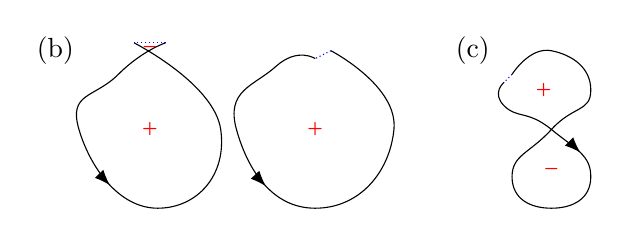
\begin{tikzpicture}[font=\tiny\boldmath\color{red}]
		\begin{scope}[scale=1, shift={(5,0)}] %around (b) and (c)
		\begin{scope}[decoration={
			markings,
			mark=at position 0.4 with {\arrow{Latex[length=2mm]};}}
		%	mark=at position 0.5 with {\arrow{>}}}
		] 
		\node at (-0.3,1) {\normalsize\color{black}(b)};
		\draw [smooth,tension=1,postaction={decorate}] plot coordinates {(1.1,1.1)(0.5,0.7)(0,0)(1,-1) (1.8,0) (0.7,1.1)};
		%\draw [smooth,tension=0,postaction={decorate}] plot coordinates {(1.1,1)(0.5,0.7)(0,0)(1,-1) (1.8,0) (0.7,1.1)};
		\draw [blue, densely dotted] (1.1,1.1) -- (0.7,1.1);
		%\draw plot [smooth,tension=0] coordinates {(1,0.9)(0.5,0.5)(0,0.2)(0,0)(1,-1) (2,0) (1.2,1)};
		\node at (0.9,1.05) {$-$};
		\node at (0.9,0) {$+$};
		
		\begin{scope}[shift={(2,0)}]
		\draw [smooth,tension=1,postaction={decorate}] plot coordinates {(1,0.9)(0.5,0.8)(0,0)(1,-1) (2,0) (1.2,1)};
		\draw [blue, densely dotted] (1.2,1) -- (1,0.9);
		%\draw plot [smooth,tension=0] coordinates {(1,0.9)(0.5,0.5)(0,0.2)(0,0)(1,-1) (2,0) (1.2,1)};
		\node at (1,0) {$+$};
		\end{scope}
		\end{scope}
		\begin{scope}[shift={(5,0)},decoration={
			markings,
			mark=at position 0.24 with {\arrow{Latex[length=2mm]};}}]
		\draw [smooth, tension=1,postaction={decorate}] plot coordinates{(0.4,0.6)(0.4,0.3)(1,0)(1.5,-0.6)(1,-1)(0.5,-0.6)(1,0)(1.5,0.5)(1,1)(0.5,0.7)};
		\draw [blue, densely dotted] (0.5,0.7) -- (0.4,0.6);
		%\draw plot [smooth,tension=0] coordinates {(1,0.9)(0.5,0.5)(0,0.2)(0,0)(1,-1) (2,0) (1.2,1)};
		\node at (0.9,0.5) {$+$};
		\node at (1,-0.5) {$-$};
		\node at (0,1) {\normalsize\color{black}(c)};
		
		\end{scope}
		\end{scope}%around (b and c)
		\end{tikzpicture}	
		\caption[Demonstrations of signed area]{\label{fig:winding} (a) A complicated closed path showing the multiplicity of each region it contains, (b) two idealised handwritten digit 0s showing the completion into a closed curve and showing how the nature of the straight line completion has only a small effect on the area, and (c) an illustration of an idealised handwritten digit 8 showing why, although it is a large object, its area might be small due to cancellation of a positive and negative part.}
	\end{center}
\end{figure}


As an example of how the area can be useful in classifying the shape of the path, consider classifying handwritten digits 0 and 8. Usually these are written with a single stroke which ends near its beginning, so the displacement is insufficient for distinguishing them. This is reflected in Figure~\ref{fig:displacement} which shows the 0s and 8s near the origin and intermingled. However, the signed areas are statistically different. The figure 0 is typically formed from a single anticlockwise loop, generating a positive signed area, while the figure 8 contains two regions with opposite sign, leading to cancellation of signed area. The diagrams in Figure~\ref{fig:winding}(b) and (c) illustrate this. 
%The Pendigits dataset \cite{pendigits} collected the traces of many people writing the digits 0 to 9, and 
The histogram in Figure~\ref{fig:histogram80} shows how different the  signed areas of the first (and usually only) strokes of these digits are for the same Pendigits training data.
This clear separation is an illustration of the potential usefulness of the signature for machine learning.
\begin{figure}[H]
	\begin{center}
		\includegraphics[width=4.387in]{histogram80}
		\caption[Histogram of Pendigits 8 and 0 first stroke signed areas]{\label{fig:histogram80}Histogram of areas of the first stroke of each 0 and 8 in the training portion of the Pendigits dataset.}
	\end{center}
\end{figure}

I discuss later some extensions to the idea of signed area. In \autoref{sec:myInvariant} I discuss a generalisation of this concept of signed area to more than two dimensions, and in \autoref{chap:aoa} I discuss interpreting the whole signature, or large parts of it, as signed areas calculated recursively.

\section{Words}
\label{sec:words}
In this section I introduce some background algebraic structures which I refer to repeatedly later.
The main source for all this background is \cite{FLA}. An informal introduction is given in \cite{LOGSIG}.
Consider a set $\Sigma=\{\alph{1},\alph{2},\dots,\alph{d}\}$\jindmath{\alph{1},\alph{2},\dots,\alph{d}}{12345} of $d$ ``letters'' which has an ordering $<$\jindmath{<}{<}. I use these blue bold numbers as labels for the dimensions. %, such as the set of upper case letters $A,\dots,Z$ or the numbers $\alph{1},\alph{2},\alph{3}$. 
The set of words with entries in $\Sigma$\jindmath{\Sigma}{Sigma} is called the \emph{Kleene Star} of $\Sigma$ and is denoted by $\Sigma^*$\jindmath{\Sigma^*}{Sigmas}. 
The length of a word $u$ is denoted $|u|$\index{u@$\vert u\vert$}. %this is a special use of " to quote index characters 
The empty word is denoted by $\emptyword$\jindmath{\emptyword}{epsilon} and the concatenation of words $u$ and $v$ is written $uv$%; concatenation is an associative operation
. If a word $w$ is equal to $uv$ for some words $u$ and $v$, then $u$ is said to be a \emph{prefix} of $w$ and $v$ is said to be a \emph{suffix} of $w$. If $u$ and $v$ are both not empty then they are said to be a \emph{proper} prefix and suffix of $w$. For example $\alph{1}$ is a proper suffix of $\alph{3231}$, and a suffix but not a proper suffix of $\alph{1}$.
The ordering $<$ on $\Sigma$ can be extended to an ordering $\lex$ \jindmath{\lex}{< <}on $\Sigma^*$ called \emph{alphabetical order} or \emph{lexicographic order} in the usual way. (Specifically: $\emptyword\lex u$ if $|u|>0$. For letters $a$ and $b$ and words $u$ and $v$, $au\lex bv$ if $a<b$ or both $a=b$ and $u\lex v$.)

%\section{Free vector space}
The \emph{free (real) vector space} on the finite set $\Sigma$ is the real vector space with basis given by the elements of $\Sigma$. We will just call it $\mathbb{R}^d$. An element looks like $a_1\alph{1}+\dots+a_d\alph{d}$ for real numbers $a_1,\dots,a_d$.

%\section{Tensor algebra}
The \emph{tensor algebra} of the vector space $\mathbb{R}^d$,  $\TS$\jindmath{\TS}{T}, is the set of finite sums of real multiples of words, or equivalently the set of functions from $\Sigma^*$ to $\mathbb{R}$ which are zero for all but finitely many words, or equivalently the free vector space on $\Sigma^*$, $\R\langle\Sigma\rangle$. $\TC$\jindmath{\TC}{TT} denotes the  functions from $\Sigma^*$ to $\mathbb{R}$, or formal power series on $\Sigma$ considered as noncommuting, or equivalently the set of (possibly) infinite formal sums of real multiples of words, $\R\langle\langle\Sigma\rangle\rangle$.  The word $u$ in $\Sigma^*$ is identified with the function which takes $u$ to 1 and all other words to 0, or the expression $1u$. 
We are only ever interested in finite restrictions of these in order to do calculations, in particular we choose an integer $m$ and ignore all words with length longer than $m$. $T^{\underline m}(\mathbb{R}^d)$\index{Tm@$T^{\underline m}(\mathbb{R}^d)$} is the real vector space with basis given by words of length $m$ or less\footnote{this is known as $T^{(m)}(\mathbb{R}^d)$ in the notation of \cite{Lyons07}}. 
%The function on pairs of words which returns their concatenation if it has length $m$ or less and returns the zero element otherwise extends uniquely to a bilinear operation\footnote{i.e. linear in each argument} on $T^{\underline m}(\mathbb{R}^d)$, which is called the \emph{concatenation product}. 
%Given two words $w_1$ and $w_2$, their concatenation is the word $w_1w_2$
The concatenation of words is extended linearly to form bilinear\footnote{i.e.~linear in each argument} associative operations on $\TC$, $\TS$ and $T^{\underline m}(\mathbb{R}^d)$ called the \emph{concatenation product}.
(On $\TC$ this is well defined and doesn't involve calculating infinite sums because each word is only the concatenation of finitely many pairs of words.)
For example, in $T^{\underline 4}(\mathbb{R}^3)$,\footnote{because the concatenation of $\alph{132}$ and $\alph{21}$ is ignored}
\[(9\emptyword+7\,\alph{132})(2\,\alph{1}+4\,\alph{21})=18\,\alph{1}+36\,\alph{21}+14\,\alph{1321}.\]

Level $m$ of the signature can be thought of as taking values in $(\mathbb{R}^d)^{\otimes m}$, which is a $d^m$-dimensional real vector space. In this form, the signature is seen to be an element of $\TC$.
If $a\in\TS$ and $b\in\TC$ we can form the inner product $\langle a,b\rangle=\langle b,a\rangle$\index{<>@$\langle,\rangle$} in the word basis because this is only a sum over the finitely many terms in $a$. In this way $\TS$ is a set of linear maps $\TC\to\R$. If $a\in\TS$ and $X$ is a signature then the notations $X(a)$ and $\langle a,X\rangle$ are equivalent for the value of the signature on $a$.\footnote{There is a slight confusion with the term ``signature element'', as it is used for both the value of a signature on an $a\in\TS$ and also, sometimes, specifically for the value of a signature on a word.}

If $p$, $q$ and $r$ are real numbers with $p<q<r$ and $\gamma$ is a bounded variation path $[p,r]\to \R^d$ then the result (from \cite{chen}) known as \textbf{Chen's identity} states that \begin{equation}
X^\gamma_{p,r}(i_1i_2\ldots i_n) %$
=\sum_{j=0}^nX^\gamma_{p,q}(i_1i_2\ldots i_{j})X^\gamma_{q,r}(i_{j+1}i_{j+2}\ldots i_n).
\end{equation}
(The products indicated with ellipses can be empty, indicating the empty word, on which any signature takes the value 1.) 

Restricting up to level $m$, this means that 
\begin{equation}\label{eq:chenInIntro}
X^{\gamma,\underline m}_{p,r}=X^{\gamma,\underline m}_{p,q}X^{\gamma,\underline m}_{q,r},
\end{equation}
using the concatenation product in $T^{\underline m}(\mathbb{R}^d)$, where $X^{\gamma,\underline m}_{p,r}$ means the signature of $\gamma$ on $[p,r]$ up to level $m$.

%\subsubsection{Shuffle product}

Given two words $w_1$ and $w_2$, their shuffle product $w_1\shuffle w_2$ \jindmath{\shuffle}{sha} is the multiset of words which can be formed by interleaving them, including multiplicity, which we write as a polynomial on words. For example
\begin{align*}
\alph1\alph2\shuffle\alph3 &= \alph3\alph1\alph2+\alph1\alph3\alph2+\alph1\alph2\alph3
\end{align*}
This is extended linearly to a commutative and associative operation on $\TS$.

The signature $X$ of a bounded variation path obeys the following relation, for any $a,b\in\TS$, which is a consequence of integration by parts or the product rule for differentiation. (\cite{Ree}, see also \cite[Theorem 3.2]{FLA})
\begin{equation}\label{eq:shuffle}
X(a)X(b)=X(a\shuffle b)
\end{equation}
In particular, therefore, not every element of $\TC$ is the signature of a bounded variation path. For example, we see that $X(\emptyword)$ must be $1$. Allowed elements are those known as \emph{grouplike} elements.\footnote{This is equivalent to the remark in section~3.5.2 of \cite{FLA}.}


\section{What is the log signature of a path?}
\label{sec:logsigs}
The \emph{log signature} (\cite{Sidorova}, \cite{Lyons07}, also \emph{logarithmic signature}) is a compressed version of the signature. 
It carries the same information, but in a more compact way. 
It is also divided into levels. 
Up to level $m$, the log signature contains fewer numbers than the signature.
Any given set of values for these numbers actually gives the log signature of some path up to that level, whereas 
this is not the case for signatures, because there is some redundancy in the signature.
For example the first two levels of the signature of a two-dimensional path consists of $2+2^2=6$ numbers but we saw that this information is the path's total displacement and signed area, which can be stored in three numbers, which are exactly the first two levels of the log signature. In applications, the log signature might be less susceptible to roundoff error. The log signature is defined in terms of the signature, in a way analogous to logarithms of numbers, but can be calculated via an independent algorithm.

%Any machine learning example where log signatures beat signatures
 
 
%\section{Log Signatures}
The space $\TC$, in which the signature of a $d$-dimensional path lives, has a notion of logarithm (\cite{FLA}, chapter 3), given by 
\begin{equation}\label{eq:log}
\log(\emptyword+T)=\sum_{n\ge1}\frac{(-1)^{n-1}T^n}{n},\jind{log}
\end{equation}
where $T$ has no $\emptyword$ component, and a notion of exponential, given by 
\begin{equation}\label{eq:expDef}
\exp(T)=\emptyword+\sum_{n\ge1}\frac{T^n}{n!}.\jind{exp}
\end{equation}
In particular, these are well-defined operations which are inverses
\begin{equation}
\big\{x\in T^{\underline m}(\mathbb{R}^d) \mid \langle x,\emptyword\rangle=1\big\}
\underset{\log}{\overset{\exp}{\leftrightarrows}}
\{x\in T^{\underline m}(\mathbb{R}^d) \mid \langle x,\emptyword\rangle=0\}.
\end{equation}
%where powers are in the concatenation product
%The signature itself lies on a submanifold of tensor space.
%Calculating the log signature expanded
Let $S$ be the set which consists of the signature of every path in $\mathbb{R}^d$ truncated up to some level $m$.
$S$ is not the whole of the vector space  $T^{\underline m}(\mathbb{R}^d)$, although it does \textit{span}  $T^{\underline m}(\mathbb{R}^d)$
%\footnote{see Lemma 8 in \cite{JD}}. 
(see \cite[Lemma 8]{JD}). In fact, $S$ forms a lower-dimensional manifold. The 
logarithm operation %(\cite{FLA}, chapter 3) %$\log:T(\mathbb{R}^d)\to T(\mathbb{R}^d)$ is defined by $\log(1+T)=\sum_{n\ge1}\frac{(-1)^{n-1}T^n}{n}$. 
maps this manifold continuously one-to-one to a linear subspace of $T(\mathbb{R}^d)$.
%(Note: as formal series, it is not true that the logarithms of all signatures of paths without truncation form a linear subspace.)
The image of a signature under the logarithm or its representation in a basis of this subspace is called the \textbf{log signature}. %The log signature of a path up to level $m$ is determined by an easy calculation from its signature up to level $m$, and t
The logarithms of two signatures which agree up to level $m$ will agree up to level $m$, and so the phrase ``log signature of a path up to level $m$'' is unambiguous.
%The passage to the log signature can be considered an information compression or a dimensionality reduction. 

The subspace in which the log signature of a path in $\mathbb{R}^d$ up to level $m$ lives is equivalent to the free $m$-nilpotent Lie algebra of type $d$, $\mathfrak{n}_{d,m}$. The log signature is a completely compressed version of the signature up to the same level -- for every value in $\mathfrak{n}_{d,m}$, there is a path with that truncated log signature. It is a Lie algebra under the bracketing operation defined by $[a,b]=ab-ba$. A clear presentation of the background to this is found in \cite{LR}.

$\mathfrak{n}_{d,m}$ is a finite dimensional real vector space, but there is no single obvious basis for it. In order to use the log signature as an efficient representation of a path, we need to choose a fixed basis.
%We return the log signature in terms of a fixed basis, so that it can be used as an efficient representation of a path. 
There are two commonly used bases. They are both \emph{Hall bases}\cite{hall1950}. A Hall basis is made up of bracketed expressions, which are expressions involving letters combined with Lie brackets like $[\alph1,[\alph2,\alph1]]$, and it is determined by an ordering of all bracketed expressions.
\begin{itemize}
	\item The \emph{Lyndon basis}\cite{shirshov}. Each basis element is labelled with a Lyndon word on $\{\alph1,\alph2,\dots,\alph{d}\}$, which is a sequence which comes earlier in lexicographic order than any of its \emph{rotations}. (For example, the rotations of $\alph{2432}$ are $\alph{2243}$, $\alph{3224}$ and $\alph{4322}$. $\alph{2243}$ and $\alph{1213}$ are Lyndon words but $\alph{31}$ and $\alph{3224}$ are not.) %in which each Lyndon word is the foliage of exactly one basis element. Within each level, we order the basis elements so that their Lyndon words are in alphabetical order.
	\item The standard/canonical Hall basis, which we implement in such a way as to match CoRoPa\cite{coropa} exactly. %This basis still has the property that each element can be identified by its foliage
	The ordering of equal-length expressions $[A,B]$ and $[C,D]$ is defined recursively: $[A,B]<[C,D]$ if either $A<C$ or ($A=C$ and $B<D$).
\end{itemize}

In these bases, each basis element is either a letter or a single bracketed expression, whose left and right are basis elements. We always pick an order on basis elements such that shorter bracketed expressions come before longer ones, and single letters, which are the first level, are in their natural order $\alph1<\alph2<\dots<\alph{d}$.

From each bracketed expression we can form a word by deleting the brackets, which we call the expression's \emph{foliage}. For example the foliage of $[\alph1,[\alph2,\alph1]]$ is $\alph{121}$. Elements of a Hall basis are labelled by their foliages, which are called \emph{Hall words}. In the Lyndon basis the Hall words \emph{are} the Lyndon words.

In summary, the signature of a path is a special type of element of tensor space, called a grouplike one. It is the tensor exponential of a Lie element. 
This element is called the \emph{log signature} of the path.
Hall bases are practical bases for free nilpotent Lie algebras, which is where truncated log signatures take their values.
A Hall basis is graded, its elements in each level provide a basis for that level. Its elements in level $m$ are labelled with words of length $m$ called Hall words.
The term \emph{log signature} of a path is also used for the numerical expression in terms of a Hall basis.
If $h$ is a Hall word, we write $P_h$ for the corresponding Lie element.\jindmath{P_\cdot}{P}
%This notation assumes that a particular Hall basis is fixed. 

\subsection{Extracting a single log signature element from the signature}
\label{sec:usepi1adjoint}
Every polynomial function on signatures can be written uniquely as a linear combination of signature elements, i.e.~as a linear function on the signature. In particular, any element of the log signature can be written as an expression in terms of the signature. 
Here I present a simple way to find this expression.%, which was suggested by Joscha Diehl.

Considering everything up to level $m$, there is a unique linear map $\pi_1$\jindmath{\pi_1}{pi1} defined on the truncated tensor algebra which agrees on truncated grouplike elements with the logarithm function. This is explained on page 58 of \cite{FLA}. %It is not the easiest thing to calculate, but 
%We write down an expression for its transpose, which is efficient to calculate in practice.
(This is an example of the general principle that every polynomial function from grouplike elements / signatures to the reals extends uniquely to a linear function from $\TC$ to the reals. This reflects how much redundancy there is in the signature.).

%I note some local definitions from \cite{FLA}.
Denoting the non-empty words by $\Sigma^+$, $\pi_1$ of a word $w$ is given by 
\begin{align}
\pi_1(w)=\sum_{k\ge1}\frac{(-1)^{k-1}}{k}\sum_{u_1,\dots,u_k\in \Sigma^+}\langle w,u_1\shuffle\dots\shuffle u_k\rangle u_1\cdots u_k.\label{eq:pi1}
\end{align}
Its adjoint $\pi_1^\top$ \jindmath{\pi_1^\top}{pi1t}, which \cite{FLA} introduces in section 6.2 as $\pi_1^*$, is given by the similar expression, using the duality between shuffle and concatenation.
\begin{align}
\pi_1^\top(w)=\sum_{k\ge1}\frac{(-1)^{k-1}}{k}\sum_{u_1,\dots,u_k\in \Sigma^+}\langle w,u_1\cdots u_k\rangle u_1\shuffle\dots\shuffle u_k \label{eq:pi1adjoint}
\end{align}
This is explained in section~IV of \cite{Kawski}, where $\pi_1^\top$ is called $\pi_1'$.
$\pi_1^\top$ is easier to calculate than $\pi_1$ because its inner sum is simply over all decompositions of $w$ into $k$ words without having to think about preimages of the shuffle product.

For example,
\begin{align*}
\pi_1^\top(\alph{112})=\alph{112}-\frac12(\alph1\shuffle\alph{12}+\alph{11}\shuffle\alph2)+\frac13\alph1\shuffle\alph1\shuffle\alph2
\end{align*}

Fixing a Hall basis, there is a well known basis of each level of tensor space called the Poincar\'e-Birkhoff-Witt basis or PBW basis, described around page~91 of \cite{FLA}. Each basis element of level $m$ is indexed by a word of length $m$, we use the notation $P_w$\jindmath{P_\cdot}{P} for the element indexed by the word $w$. The PBW basis has the property that when $w$ is a Hall word then $P_w$ is the corresponding Lie element. 
Thus the notation here is consistent with our use of $P_w$ above when $w$ is a Hall word. 

On page~108 of \cite{FLA} is given an explicit construction of a dual basis $S$\jindmath{S_\cdot}{S} for the PBW basis. This is indexed by words, and if $w$ is a word then both $S_w$ and $P_w$ are elements of level $|w|$ of the tensor algebra. In particular, for any words $w$ and $w'$ we have that $\langle S_w,P_{w'}\rangle$ is 1 if $w=w'$ and zero otherwise.\footnote{Angle brackets are always the inner product in the word basis described in \autoref{sec:words}.}

%We can now 
%Let the log signature of a path be given by $l_\cdot$, i.e.~as $\sum_{h \text{ Hall}}l_hP_h$, and lets say we wish
Let's say we wish to find an expression for the log signature element corresponding to the basis element labelled with Hall word $h$.
If $X$ is the signature, then because its logarithm can be written as $\log X=\sum_{h' \text{ Hall}}l_{h'}P_{h'}$ for constants $l_\cdot$ and we are looking for $l_h$, our target is %we are actually looking for an expression for 
\begin{align}
\langle S_{h},\log X\rangle=\langle S_{h},\pi_1(X)\rangle=\langle \pi_1^\top(S_{h}),X\rangle
\end{align}
Thus $\pi_1^\top(S_{h})$ is exactly the expression we need.
This is not used in any of this work but is a possible alternative for obtaining the log signature whose performance could be investigated.

\subsection{An illustration}
  The log signature up to level 4 has 8 degrees of freedom. We can write it as tensors in the Lyndon basis in the following general form.%, writing $a\alph1$ as a short form for $aP_{\alph1}$ and so on.
\begingroup
\def\negjr#1{\ifnum\pdfstrcmp{0}{#1}=0 0 \else -#1\fi}
\def\pbinomjr#1#2{\left(\begin{smallmatrix}#1\\#2\end{smallmatrix}\right)}
\def\tr#1#2#3{\left(\begin{smallmatrix}#1\\#2\\#3\end{smallmatrix}\right)}
\def\ttr#1#2#3{\left(\begin{smallmatrix}0&#1&#3\\\negjr{#1}&0&#2\\\negjr{#3}&\negjr{#2}&0\end{smallmatrix}\right)}
\def\tttr#1{\left(\begin{smallmatrix}#1\end{smallmatrix}\right)}
\renewcommand\arraystretch{1.33}
\def\w#1{\makebox[\widthof{$\scriptstyle a^2b^2+4abc+12ae+12bd+214g-48g$}][c]{$\scriptstyle #1$}}
\begin{align}\begin{array}{c @{{}+{}} c @{{}+{}} c @{{}+{}} c}
    %a\alph1+b\alph2 & c\alph1\alph2 & d\alph1\alph1\alph2+e\alph1\alph2\alph2 & f\alph1\alph1\alph1\alph2+g\alph1\alph1\alph2\alph2+h\alph1\alph2\alph2\alph2\\
    aP_{\alph1}+bP_{\alph2} & cP_{\alph1\alph2} & dP_{\alph1\alph1\alph2}+eP_{\alph1\alph2\alph2} & fP_{\alph1\alph1\alph1\alph2}+gP_{\alph1\alph1\alph2\alph2}+hP_{\alph1\alph2\alph2\alph2}\\
    %a\alph1+b\alph2 & c[\alph1,\alph2] & \begin{matrix}d[\alph1,[\alph1,\alph2]]\\+\\e[[\alph1,\alph2],\alph2]\end{matrix} & f\alph1\alph1\alph1\alph2+g\alph1\alph1\alph2\alph2+h\alph1\alph2\alph2\alph2\\
    \pbinomjr{a}{b}& \tttr{0&c\\-c&0} & \tttr{\tttr{0&d\\-2d&e}\\\tttr{d&-2e\\e&0}} & \left(\begin{smallmatrix}\tttr{\tttr{0&f\\-3f&g}\\\tttr{3f&-2g\\0&h}}\\\tttr{\tttr{-f&0\\2g&-3h}\\\tttr{-g&3h\\-h&0}}\end{smallmatrix}\right)
\end{array}.\label{eq:arblogsig}
\end{align}
When exponentiated using \eqref{eq:expDef}, this expresses the signature truncated up to level 4 in the following form
\begin{align}
    &1+\pbinomjr{a}{b}+\tfrac12\left(\begin{smallmatrix}a^2&ab+2c\\ab-2c&b^2\end{smallmatrix}\right)
    +\tfrac16\tttr{\tttr{\makebox[\widthof{$\scriptstyle ab^2+6e+3bc$}][c]{$\scriptstyle a^3$}&a^2b+6d+3ac
      \\a^2b-12d& ab^2+6e+3bc}
    \\\tttr{a^2b+6d-3ac&ab^2-12e
      \\ab^2+6e-3bc&\makebox[\widthof{$\scriptstyle ab^2+6e+3bc$}][c]{$\scriptstyle b^3$}}}\nonumber
  \\&+\tfrac1{24}\left(\begin{smallmatrix}\tttr{\tttr{\w{a^4}&\w{a^3b+4a^2c+12ad+24f}\\a^3b-12ad-72f&a^2b^2+4abc+12ae+12bd+24g}\\\tttr{\w{a^3b-12ad+72f}&a^2b^2+4abc-24ae-24bd+12c^2-48g\\a^2b^2+24ae-12c^2&ab^3+4b^2c+12be+24h}}\\\tttr{\tttr{a^3b-4a^2c+12ad-24f&a^2b^2+24bd-12c^2\\a^2b^2-4abc-24ae-24bd+12c^2+48g&\w{ab^3-12be-72h}}\\\tttr{a^2b^2-4abc+12ae+12bd-24g&ab^3-12be+72h\\\w{ab^3-4b^2c+12be-24h}&\w{b^4}}}\end{smallmatrix}\right)\label{eq:arbsig}
\end{align}
Writing this out in terms of words would look like
\begin{align} \emptyword+a\alph1+b\alph2+\frac12\Big[a^2\alph{11}+(ab+2c)\alph{12}+(ab-2c)\alph{21}+b^2\alph{22}\Big]+\cdots
\end{align}
\endgroup

\endDocumentJR
